\chapter{Kociemba's Optimal Solver}
\label{chap:kociembaImplement}
\myTop{The actual implementation of Kociemba's optimal solver will be covered in this chapter. The reader will be presented with general description of how we have chosen to implement Kociemba's optimal solver along with a detailed explanation of key points of the source code.}
The basics of Kociemba's optimal solver have been covered in section \ref{sec:kociemba}. The algorithm which we are implementing differs from the original at one point:
We are interested in the shortest move sequence to solve a scrambled cube, whereas the original Kociemba optimal solver only finds the shortest length, not the actual sequence of moves \cite{rokicki09}.

Because of this we have chosen not to have a lookup table since it would have to contain 20 billion move sequences, which is impossible on today's computers. Considering that the lookup table only contains the length, it would have a size of 4 GB \cite{cubeExplorer}. A table containing the move sequences would have to be much larger.

An $A$ move can be defined using 4 bits.
The 4 bits gives $2^4=16$ different spaces and there are 10 $A$ moves, which mean they will fit.
To calculate the size of a lookup table containing the move sequence is just a matter of multiplying the size of one move with the number of moves in a sequence, e.g. a move sequence of the length 14 would have the size: $4 \cdot 14 = 56$ bits.
This size is again multiplied with the number of positions which needs this length for solving.
The size of a lookup table containing every move sequences to solve the \rubik{} inside \m{H} would be: $987$ GB (see appendix \ref{chap:sizeOfLookup}), which exceeds the average memory on today's computer \cite{averageRAM} \cite{maxRAM2}.

Instead of the lookup table our solver will have to try every move sequence inside \m{H} and find the one with the shortest length. A flowchart of our implementation is shown in figure \ref{fig:kociembaFlow}.  As in the flowchart $b$ is a move sequence variable, which takes the scrambled cube into \m{H}. $d$ is the depth, i.e. the number of moves in $b$, $c$ is the move sequence which solves the cube when it gets inside \m{H}, and $e$ is the depth which the \m{H} solver is searching. $result$ is the shortest move sequence found to solve the cube, this is updated every time a shorter move sequence is found.

\begin{figure}[htbp]
	\centering
		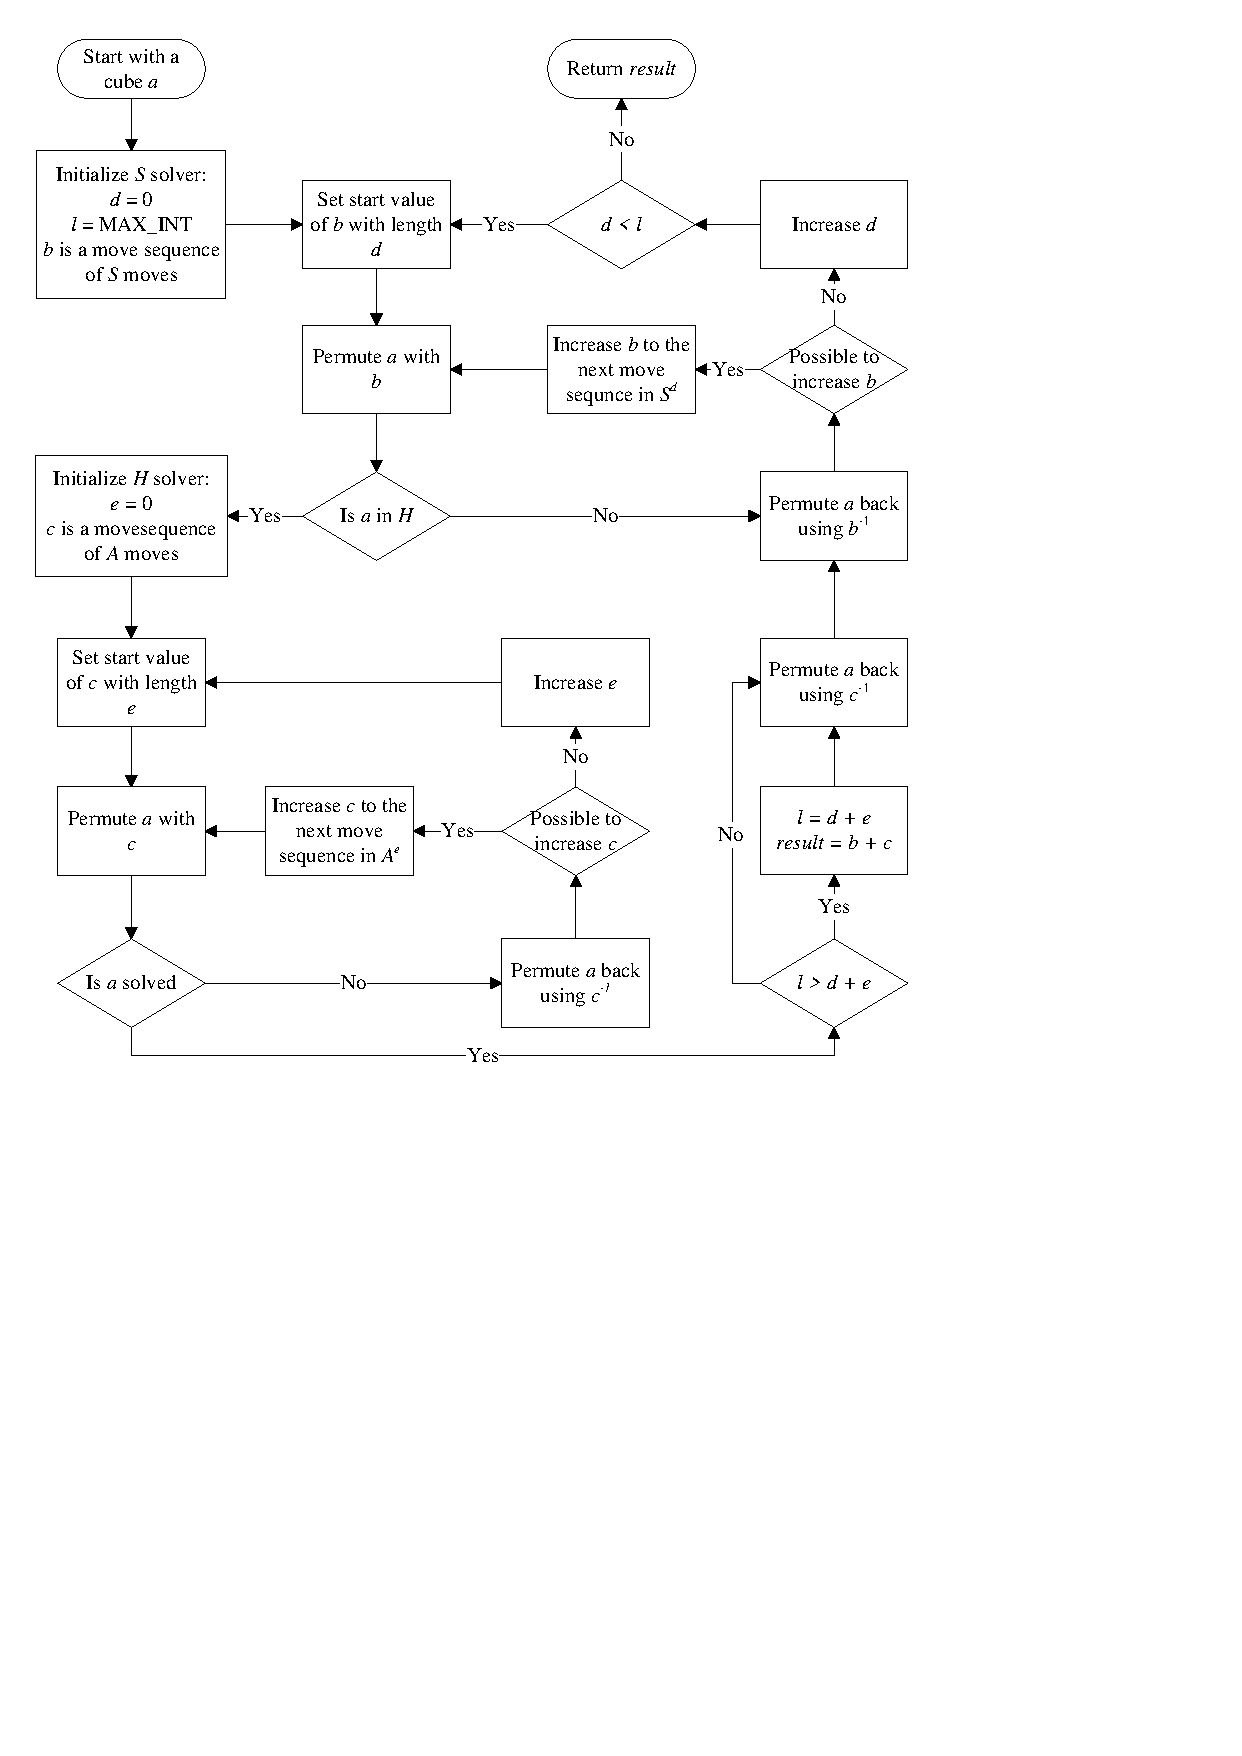
\includegraphics[width = \textwidth, trim = 0mm 110mm 50mm 0mm, clip]{input/pics/kociembaFlow}
	\caption{\myCaption{A flow chart of our implementation of Kociemba's optimal solver.}}
	\label{fig:kociembaFlow}
\end{figure}

	\section{Incrementing a Move Sequence}
\label{sec:incMoveSequence}
Our implementation of the Kociemba's optimal solver will be incrementing move sequences.
This means that the move sequence will be changed to the next in a given set.

E.g. if the move sequence which is about to be incremented is \m{F R'} and the set which is being incremented in is \m{S}, then incrementing it will change the last move \m{R'} to the next \m{R2} -- hence the new move sequence \m{F R2}.
This is very similar to incrementing an integer by hand; the last digit will become the next number in the decimal system until the last digit is 9. When this happens the second last digit is increased by one and the last digit is set to be the first number in the decimal system: 0.

So when our move sequence \m{F R2} is being incremented \m{R2} will become \m{U}, since \m{R2} is the last move in the set of moves \m{S}. \m{F} will then be increased to \m{F'}, this gives the new move sequence \m{F' U}.
	\section{Method Solve}

- Initialiserer 5 variabler af forskellige typer
- hopper ind i en while l\o{}kke
- hvergang while l\o{}kke bliver k\o{}rt bliver et array initialiseret lavet af moves.
- twist
- to moves af samme type
-  humle = pilsen knappes
- hopper ind i l\o{}kke der k\o{}rer uendeligt
- hvor den permuter med moveseq b
- k\o{}rer lignende funktion , som hedder solveFromH
- g\o{}r den med en parameter l - d
- resultat den f\aa{}r s\ae{}tter den = c
- tester om den nuv\ae{}rende l\ae{}ngde d + l\ae{}ngden c < l
- hvis ja l = de to foreg\aa{}ende l\ae{}ngder
- initialiserer resultat arrayet
- tilf\o{}jer moveseq b og moveseq c til moveseq resultatet
- permuter cuben tilbage igen, inverse af b

- increasewithSnotendwithA --> reference
- t\ae{}ller d op
- returner resultatet i sidste ende.
-  og der er nogle try catch som s\o{}rger for at det hele ikke l\o{}ber i endless loop

The method Solve is the method that connects all the submethods into one big method that apply the Kociemba's algorithm onto the \rubik{}. It start with initializing five variables; a result array which will contain the final move sequence, a d integer which will determine the search depth, a l integer which also is used to determine the search depth, a b array which will contain the move sequence until the \rubik{} enters H and a c array which will be the move sequence after the \rubik{} has entered H. Thereafter it enters a while loop which initialize an array of moves everytime the loop runs. Thereafter the method enters a while loop which runs in a endless loop where it permutes with the move sequence b. The permute method BLALABLABLA. After that it will try solve the \rubik{} from H with the method of the same name, solveFromH, with the parameter l - d.  This will return a result that will be putted in the c array. Thereafter it test if the length d + c's length is lower than the length of l. If that is true the case l will be set as the product of d + c and the result array will be initialized with l. In The result array the move sequence b and the movesequence c is added. after it has tested the length the \rubik{}  permutes the b move sequence back one depth and perform the increaseWithSNotEndingWithA method which will be described in section BLABLA. After the increaseWithSNotEndingWithA method the program count d array size up by one.


\begin{verbatim}
try {
				while (true) {
					Cube.permute(cube, b);
					try {
						c = solveFromH(l - d);
						if (d + c.length < l) {
							l = d + c.length;
							result = new MoveButtons[l];
							output.addTextln("The solutions of the length " + l + ". The solution is:");
							int j = 0;
							for ( ; j < d; j++) {
								result[j] = b[j];
								output.addText(b[j] + " ");
							} 
							for (int k = 0 ; k < c.length; k++,j++) {
								result[j] = c[k];
								output.addText(c[k] + " "););
							}
							output.addTextln("");
						}

					} catch (InvalidCube e) {
					}
					
					Cube.permute(cube, MoveButtons.inverseOf(b));
					MoveButtons.inverseOf(b);					
					
					increaseWithSNotEndingWithA(b, b.length-1);
				}
			} catch (UnableToIncreaseMoveSequenceException e) {

			}
			d++;
		}
		return result;
	}
\end{verbatim}
	\section{The Move Incrementing Methods}
\label{sec:increaseWithSNotEndingWithA}
The method named \vr{increaseWithSNotEndingWithA} increments a move sequence. This means it will find the next move in the list of all moves.

When the method is called it takes two parameters, a move sequence of the type MoveButtons(ref) and an integer, \vr{i}, telling where in the move sequence the move should be incremented. The move sequence contains the so far executed moves.




%As the method initializes it creates two variables of the type integer, \vr{length} and \vr{i}.
%The variable \vr{length} is set equal to the length of the move sequence, so every time the length of the move sequence is needed the variable \vr{length} will be used.
%The variable \vr{i} is used to keep track of where in the move sequence a move is changed and it is set equal to the input integer parameter. 

\begin{lstlisting}[style=sourceCode, caption=\myCaption{Key point in the incrementing method of kociemba's optimal solver}, label=src:kociemba2]
if (i == length - 1) {
	try {
		do {
			moveSequence[i] = (MoveButtons)S.toArray()[moveSequence[i].ordinal() + 1];
		} while(A.contains(moveSequence[i]));
		try {
			if(isSameFace(moveSequence[i], moveSequence[i-1])) {
				increaseWithSNotEndingWithA(moveSequence, i);
			} else {
				Cube.permute(cube, moveSequence[i]);
			}
		} catch (ArrayIndexOutOfBoundsException e2) {
			Cube.permute(cube, moveSequence[i]);
		}
		return;
	} catch (ArrayIndexOutOfBoundsException e) {
		moveSequence[i] = F;
		i--;
		try {
			Cube.permute(cube, moveSequence[i].invert());
			moveSequence[i].invert();
		} catch (ArrayIndexOutOfBoundsException e4) {
			throw new UnableToIncreaseMoveSequenceException();
		}
		increaseWithSNotEndingWithA(moveSequence, i);
		return;
	}
}
\end{lstlisting}

The last move performed on the cube can never be an \m{A} move since \m{H} is a closed group (see section \ref{sec:subgroup}). The part of the code that increments the last move is shown in code snippet \ref{src:kociemba2}.
At first a \textbf{do-while} loop is executed. 
%If it is not working with the last another code snippet is executed and is very similar to this snippet. 
Inside this loop; the parameter \vr{moveSequence} will be updated with a move from \m{S} as long as the new move is a move from \m{A}. This ensure that the move is not ending in \m{A}.

After the loop has run a new method is called, \vr{isSameFace}, this method tests if the new move is the same as the move before this.
If they are the same (see section \ref{sec:groupDefinition}), then the method will call itself with the last move as a parameter else it will permute the cube with the current move.
When the \rubik{} has been permuted it will return and the method will end.

The method increments the move, it runs through the enumset \vr{S} (see code snippet \ref{src:enumset}, enumset \vr{S}).
When \m{R2} is reached the next increment will throw an \vr{ArrayIndexOutOfBoundsException}, this exception is caught in a \textbf{try-catch}.
When the exception is caught the last place in the move sequence array will be set equal to the move \m{F}(see code snippet \ref{src:enumset}, enumset \vr{notA}), which is the first move in the enumset.
When this happens the method will call it self on the move prior to the current. This will result in every move sequence it run through. 


%Now the counter variable \vr{i} will be decremented and the method will call itself.
%After it has increased the second last move it will return and end the method.

\begin{lstlisting}[style=sourceCode, caption=\myCaption{The definition of the enumsets S, A, and notA.}, label=src:enumset]
private EnumSet<MoveButtons> S = EnumSet.of(U, UP ,U2, D, DP, D2, F, FP, F2, B, BP, B2, L, LP, L2, R, RP, R2);
private EnumSet<MoveButtons> A = EnumSet.of(U, UP ,U2, D, DP, D2, F2, B2, L2, R2);
private EnumSet<MoveButtons> notA = EnumSet.of(F, FP, B, BP, L, LP, R, RP);
\end{lstlisting}

All this code is executed if and only if the first condition (\vr{i==length-1}) is true.
If it is false, then the method will start increasing the current move with an \vr{S} move (see code snippet \ref{src:enumset}, enumset \vr{S}).
This is done the same way as above, except there is no \textbf{do-while} loop around it since we are interested in all the moves in \vr{S}.

Then the method tests if two moves are on the same \face{}, just as it did in code snippet \ref{src:kociemba2}.
It will now test if the current move and the prior move is on the same face.
This is done with a \textbf{for} loop that counts every step from \vr{i} to the \vr{length} of the move sequence.

%We have been able to reuse the same code snippet
When the method gets to the end of the enumset \vr{S}, it will set the move to the first move in \vr{S} (see code snippet \ref{src:enumset}, enumset \vr{S}).
This is done with the same code as before, except this time it sets the move to \m{U}.

There is a similar method named \vr{increaseWithA} that uses a very similar code, this is called from the \vr{solveFromH} method.
The difference is that it increments with moves from \vr{A} (see code snippet \ref{src:enumset}, enumset \vr{A}).
It uses a \textbf{do-while} to increase the move \vr{moveSequence[i]} and then increase it again if \vr{A} contains this move just as code snippet \ref{src:kociemba} did with \vr{notA} (see code snippet \ref{src:enumset}).

\myTail{This chapter has shown how we have implemented Kociemba's optimal solver, with descriptions of key points of the source code.}